 \documentclass[t, xcolor=table]{beamer}
%\documentclass[c]{beamer}
\listfiles

\newcommand{\putat}[3]{\begin{picture}(0,0)(0,0)\put(#1,#2){#3}\end{picture}}
\newcommand*{\xMin}{-6}%
\newcommand*{\xMax}{6}%
\newcommand*{\yMin}{-6}%
\newcommand*{\yMax}{5}%
\setbeamertemplate{section in toc}[sections numbered]
\setbeamertemplate{subsection in toc}[subsections numbered]

\defbeamertemplate{subsubsection in toc}{subsubsections numbered}
{\leavevmode\leftskip=3em%
 \rlap{\hskip-3em\inserttocsectionnumber.\inserttocsubsectionnumber.\inserttocsubsubsectionnumber}%
 \inserttocsubsubsection\par}

\definecolor{kit-green}{RGB}{0, 150, 130}
\definecolor{kit-blue}{RGB}{70, 100, 170}
\definecolor{kit-lightgreen}{RGB}{140, 182, 60}
\definecolor{kit-orange}{RGB}{223, 155, 27}
\definecolor{kit-red}{RGB}{162, 34, 35}

\setbeamercolor{alerted text}{fg=kit-green}
% Darkened version: {fg=kit-green!80!black}

\mode<presentation>
{
  \usetheme[usefoot,english,cmyk,titlepage0]{KIT}
% \usetheme[usefoot]{KIT}
% \usetheme{KIT}

%%  \usefonttheme{structurebold}

  \setbeamercovered{transparent}

  %\setbeamertemplate{enumerate items}[circle]
  \setbeamertemplate{enumerate items}[ball]
%  \setbeamerfont{section in toc}{color=black}
  \setbeamercolor{section number projected}{bg=black,fg=yellow}
  \setbeamertemplate{subsection in toc}[subsubsections numbered]

}
\usepackage{tabularx}
\usepackage{pdfpages}
\usepackage{caption}
\usepackage{pbox}
\usepackage{multirow}
\usepackage{babel}
\usepackage{feynmp-auto}
\usetikzlibrary{calc}
\date{2018-07-09}
%\DateText

\newlength{\Ku}
\setlength{\Ku}{1.43375pt}

\usepackage[latin1]{inputenc}
\usepackage[TS1,T1]{fontenc}
\usepackage{array}
\usepackage{multicol}
\usepackage[makeroom]{cancel}
\usepackage{subfigure}
\usepackage{xspace}
%\usenavigationsymbols
%\usenavigationsymbols[sfHhdb]
%\usenavigationsymbols[sfhHb]
\newcommand{\verysmall}{\fontsize{6pt}{8.6pt}\selectfont}
\usepackage{siunitx}


\DeclareSIUnit\clight{\ensuremath{c}}
\DeclareSIUnit[per-mode=symbol]\GeVc{\GeV\per\clight}
\DeclareSIUnit[per-mode=symbol]\GeVcc{\GeV\per\clight\squared}
\DeclareSIUnit\fb{\femto\barn}
\DeclareSIUnit\invfb{\per\femto\barn}

\newenvironment<>{neutralblock}[1]{%
  \begin{actionenv}#2%
      \def\insertblocktitle{#1}%
      \par%
      \mode<presentation>{%
        \setbeamercolor{block title}{fg=white,bg=gray!70!black}
       \setbeamercolor{block body}{fg=black,bg=gray!50}
       \setbeamercolor{itemize item}{fg=white}
       \setbeamertemplate{itemize item}[triangle]
     }%
      \usebeamertemplate{block begin}}
    {\par\usebeamertemplate{block end}\end{actionenv}}

\newenvironment<>{redblock}[1]{%
  \begin{actionenv}#2%
      \def\insertblocktitle{#1}%
      \par%
      \mode<presentation>{%
        \setbeamercolor{block title}{fg=white,bg=red!70!black}
       \setbeamercolor{block body}{fg=black,bg=red!30}
       \setbeamercolor{itemize item}{fg=white}
       \setbeamertemplate{itemize item}[triangle]
     }%
      \usebeamertemplate{block begin}}
    {\par\usebeamertemplate{block end}\end{actionenv}}

\newenvironment<>{blueblock}[1]{%
  \begin{actionenv}#2%
      \def\insertblocktitle{#1}%
      \par%
      \mode<presentation>{%
        \setbeamercolor{block title}{fg=white,bg=blue!70!black}
       \setbeamercolor{block body}{fg=black,bg=blue!30!white!80}
       \setbeamercolor{itemize item}{fg=white}
       \setbeamertemplate{itemize item}[triangle]
     }%
      \usebeamertemplate{block begin}}
    {\par\usebeamertemplate{block end}\end{actionenv}}

\newenvironment<>{greenblock}[1]{%
  \begin{actionenv}#2%
      \def\insertblocktitle{#1}%
      \par%
      \mode<presentation>{%
        \setbeamercolor{block title}{fg=white,bg=green!70!black}
       \setbeamercolor{block body}{fg=black,bg=green!50}
       \setbeamercolor{itemize item}{fg=white}
       \setbeamertemplate{itemize item}[triangle]
     }%
      \usebeamertemplate{block begin}}
    {\par\usebeamertemplate{block end}\end{actionenv}}

\title[]{Modeling and Simulation of Load Balancing Strategies for Computing in High Energy Physics}
\subtitle{Karlsruhe Institute of Technology (KIT)}

\subtitle[Ren\'e Caspart]{\underline{\smash{Ren\'e Caspart}}${}^{1}$, Patrick Firnkes${}^{2}$, Manuel Giffels${}^{1}$, Anne Koziolek${}^{2}$, G\"unter Quast${}^{1}$, Ralf Reussner${}^{2}$, Maximilian Stemmer-Grabow$^{2}$}

\AuthorTitleSep{\relax}

\institute[]{Karlsruhe Institute of Technology (KIT), \inst{1} Institute for Experimental Particle Physics (ETP), \inst{2} Institute for Program Structures and Data Organization (IPD)}

\TitleImage[width=\titleimagewd]{Bilder/KIT-Titel}

\newlength{\tmplen}


\makeatletter
\let\@@magyar@captionfix\relax
\makeatother

\begin{document}


%%%%%%%%%%%%%%%%%%%%%%%%%%%%%%%%%%%%%%%%%%%%%%%%%%%%%%%%%%%%%%%%%%%%%%%%%%%%%%%%%%%%%%%%%%%%%%%%%%%%%%%%%%%%%%%%%%%%%%%%%%%%%%%%%%%%%%%%%%%%%%
\begin{frame}
  \maketitle
\end{frame}

%%%%%%%%%%%%%%%%%%%%%%%%%%%%%%%%%%%%%%%%%%%%%%%%%%%%%%%%%%%%%%%%%%%%%%%%%%%%%%%%%%%%%%%%%%%%%%%%%%%%%%%%%%%%%%%%%%%%%%%%%%%%%%%%%%%%%%%%%%%%%%
\AtBeginSection[]
{
\begin{frame}
\frametitle{Table of Contents}
\tableofcontents[currentsection,%currentsubsection, 
%    hideothersubsections, 
    sectionstyle=show/shaded,
    subsectionstyle=hide/hide,
]
\end{frame}
}

%%%%%%%%%%%%%%%%%%%%%%%%%%%%%%%%%%%%%%%%%%%%%%%%%%%%%%%%%%%%%%%%%%%%%%%%%%%%%%%%%%%%%%%%%%%%%%%%%%%%%%%%%%%%%%%%%%%%%%%%%%%%%%%%%%%%%%%%%%%%%%

\section*{Motivation}
\begin{frame}
    \frametitle{Motivation}
    \begin{columns}
        \begin{column}{0.45\textwidth}
            \begin{itemize}
                \item Flat computing budget model does not cover future needs for computing resources
                %\item In the future increased addition of non-HEP specific resources
            \end{itemize}
            \begin{center}
                \vskip -2ex
                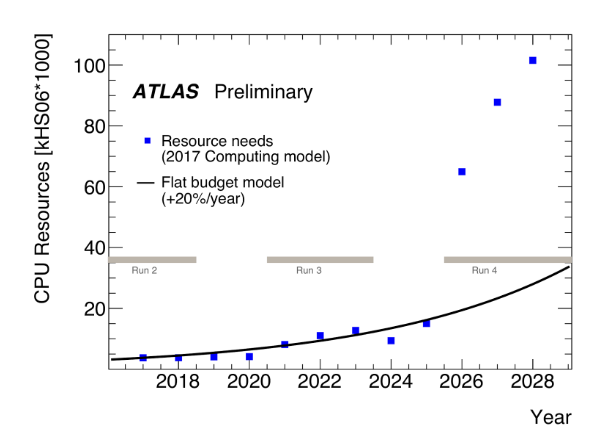
\includegraphics[width=\textwidth]{Bilder/CPU_resources_budget}
                \tiny{https://arxiv.org/abs/1712.06982}
            \end{center}
        \end{column}
        \hfill
        \begin{column}{0.5\textwidth}
            \begin{itemize}
                \item Computing resources for user jobs in HEP will be increasingly distributed and heterogeneous systems
                \item This trend can already be seen
                \begin{itemize}
                    \item Tier 2, Tier 3 and institute clusters
                    \item Addition of cloud resources like HnSciCloud and AWS
                \end{itemize}
                \item Different job types and mixtures optimal for each resource
            \end{itemize}
        \end{column}
    \end{columns}
\end{frame}

\begin{frame}
    \frametitle{Scheduling as a key component}
    \begin{columns}
        \begin{column}{0.45\textwidth}
            \begin{itemize}
                \item Already for the current resources efficient scheduling for jobs is a challenge
                \item This will become even more important for distributed heterogeneous resources in the future
                \item We need to find ways to simulate the utilization of these resources with different scheduling approaches
            \end{itemize}
        \end{column}
        \hfill
        \begin{column}{0.5\textwidth}
            \begin{center}
                \vspace{4ex}
                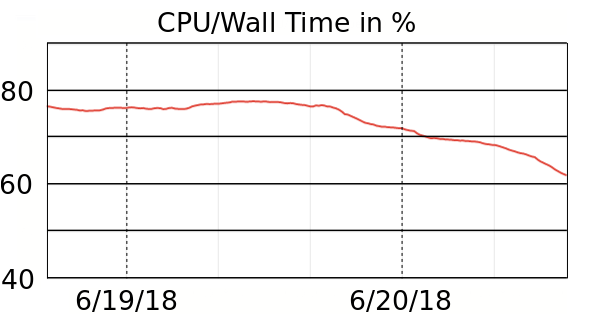
\includegraphics[width=\textwidth]{Bilder/CPU_eff_gridKa}
            \end{center}
        \end{column}
    \end{columns}
\end{frame}


\section*{Concept \& Proof of Concept}
\begin{frame}
\frametitle{Approach}

    \vspace{1em}
	\begin{itemize}
        \item Simulate the utilization of computing centers using different scheduling approaches
        \begin{itemize}
            \item Need to model workflows and resources
            \item Need to implement different scheduling approaches
            \item Check the effect of these approaches on the utilization
        \end{itemize}
        \item Make use of the \alert{Palladio} Simulator
        \begin{itemize}
            \item Established tool in the computer science community
            \item Actively developed and used by computer scientists at KIT
            \item Extended to model jobs and available resources at computing centers
        \end{itemize}
        \item As a proof of concept simulate CMS workflows at the Tier 1 center GridKa
    \end{itemize}

    
%\begin{columns}
%	\begin{column}{0.45\textwidth}
%		\begin{exampleblock}{Concept}
%		\end{itemize}
%	\end{exampleblock}
%	\end{column}
%	\hfill
%	\begin{column}{0.45\textwidth}
%	\end{column}
%\end{columns}
\end{frame}

\note[itemize]{
	\item evaluate to find best from a given set
}

\section*{Palladio Simulator}
\begin{frame}
\frametitle{Palladio Simulator}
\begin{columns}
	\begin{column}{0.45\textwidth}
		\begin{itemize}
					\setlength\itemsep{0.2em}
			\item Performance predictions for design decisions
			\item Software architecture simulator
			\item Successfully applied for
			\begin{itemize}
				\item Solving industrial problems
				\item Optimizing cloud infrastructure (chemical computing)
			\end{itemize}
			\item Abstract level: Express resource needs of jobs as statistical distributions
		\end{itemize}
	\end{column}
	\begin{column}{0.55\textwidth}
		    \vspace{4ex}
			\begin{center}
				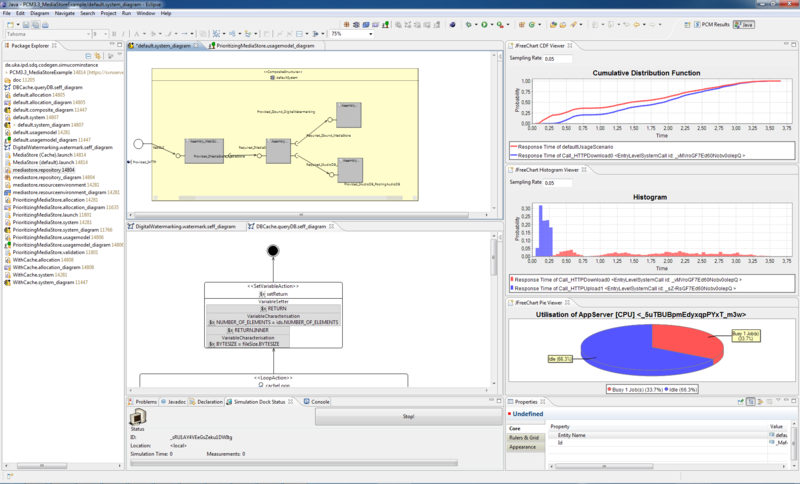
\includegraphics[width=\textwidth]{Bilder/palladio}
				\tiny{Graphical Interface of the Palladio Eclipse Plugin}
			\end{center}

	\end{column}
\end{columns}
\end{frame}

\note[itemize]{
\item Developed at KIT, FZI and University of Paderborn
\item Palladio should be used to evaluate different load balancing strategies or other design decisions (like infrastructure improvements).

\item Cloud/HEP as part of the CACTOS project

\item Architectural Templates: Enables one to efficiently model large systems (E.g. instead of modeling 1000 servers manuelly, model one server and architectural templates duplicates this server 1000 times).
\item SimuLizar: Simulate self adapting systems


}

\section*{Model Computing Jobs}
\begin{frame}
\frametitle{Model Computing Jobs}
\begin{columns}
	\begin{column}{0.45\textwidth}
		\begin{itemize}
		\setlength\itemsep{1em}
			\item Model each kind of computing job with its resource usage
				\begin{itemize}
					\item CPU \& I/O
					\item Required job slots
					\item Number of events
				\end{itemize}
			\item Model high load on system
			\begin{itemize}
				\item Closed workload
				\item Enough jobs to guarantee that systems never idles
				\item Each job type has configurable share of load
			\end{itemize}
        \end{itemize}
	\end{column}
	\hfill
	\begin{column}{0.45\textwidth}
		\begin{center}
			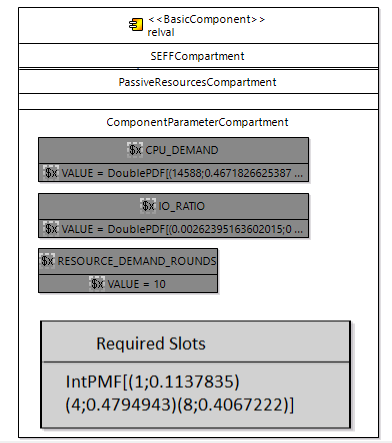
\includegraphics[width=\textwidth]{Bilder/component}
			\tiny{Screenshot: Computing job component in Palladio}
		\end{center}
	\end{column}
\end{columns}
\end{frame}

\note[itemize]{
	\item Different Models of the system are created, on for the resource environment, the assembly (how components work togehter), the usage, the allocation and the component behaviour (e.g. required resources).
	
	\item Required Resources are probability distributions
	\item Jobs block and wait for free slots if not enough job slots are available on working node.
}


\begin{frame}
\frametitle{Model Resource Container}
\begin{columns}
	\begin{column}{0.45\textwidth}
		\begin{itemize}
			\setlength\itemsep{1em}
			\item Model each type of computing node
			\begin{itemize}
				\item Number and processing speed of cores
				\item I/O capabilities
				%\item Number of job slots
				\item Number of instances of node
			\end{itemize}
			\item Model load balancing strategy
				\begin{itemize}
					\item First fit search based on available job slots
					\item Easily modifiable to evaluate new strategies
				\end{itemize}
			
		\end{itemize}
	\end{column}
	\hfill
	\begin{column}{0.33\textwidth}
		\begin{center}
			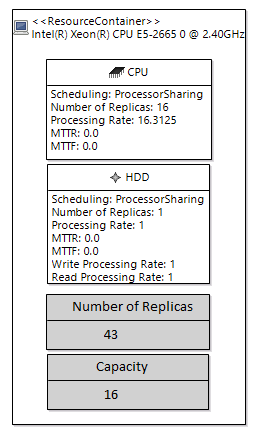
\includegraphics[width=\textwidth]{Bilder/model-container}
			\tiny{Screenshot: Resource container in Palladio}
		\end{center}
	\end{column}
\end{columns}
\end{frame}

\begin{frame}[c]
    \frametitle{Simulating CMS Jobs at GridKa}
    
    Data Sources:
    \begin{columns}
        \begin{column}{0.45\textwidth}
            \begin{itemize}
                \item Global job monitoring data
                \begin{itemize}
                    \item JobMonitoring, WMArchive job reports \\
                    {\scriptsize from Hadoop analytix cluster with CMSSpark framework (Kuznetsov)}
                    \item Currently extracting CMS jobs at GridKa
                \end{itemize}
                \item Site-specific performance data
                \begin{itemize}
                    \item VO resource share
                    \item Node benchmarks
                \end{itemize}
            \end{itemize}
        \end{column}
        \begin{column}{0.45\textwidth}
            \begin{center}
            {\scriptsize Realistic job CPU usage profiles \\ (including failing jobs)}

            \vspace{0.5em}

                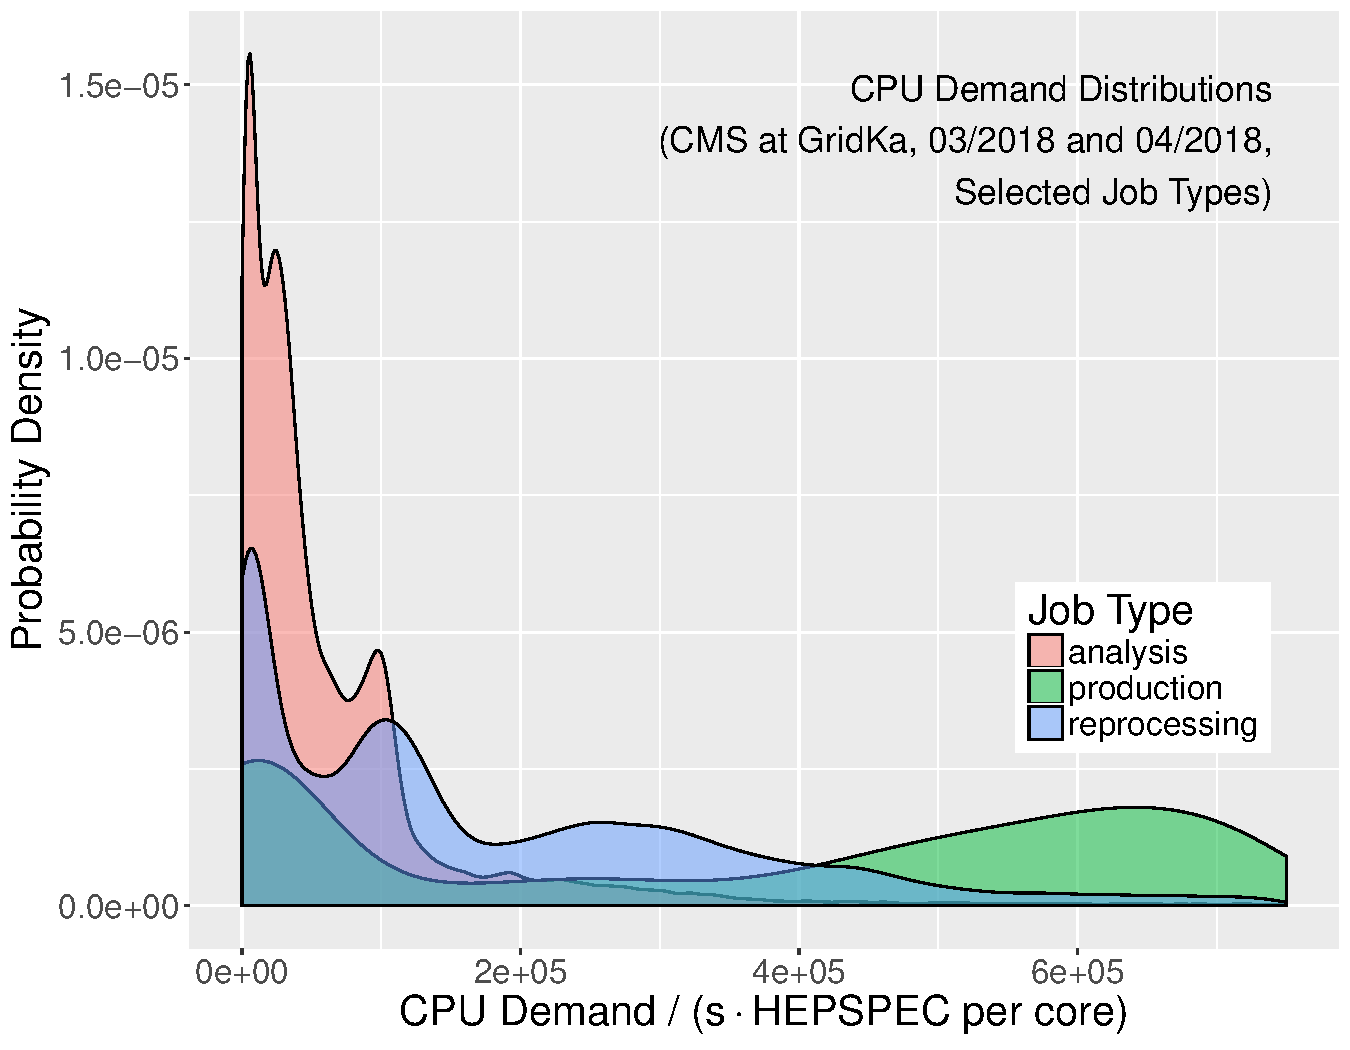
\includegraphics[width=\textwidth]{Bilder/histogram_CPUDemand_all-2018-03to04}
            \end{center}
        \end{column}
    \end{columns}

\end{frame}

\note[itemize]{
    \item Model relies on accurate laod and job resource requirement descriptions
    \item Matching job reports from different subsystems heuristically due to differing monitoring record structures
    \item Simulation model is being generated from extracted model parameters
}

\begin{frame}[c]{Model Calibration Process}
    \begin{columns}
        \begin{column}{0.45\textwidth}
            \setbeamertemplate{enumerate items}[default]
            
            Automated parameter extraction:
            \vspace{1em}
            \begin{enumerate}
                \item \alert{Match} jobs and node performance information
                \item \alert{Group} computing jobs by type and requirements
                \item \alert{Extract} resource demand distributions and load composition
            \end{enumerate}

            
        \end{column}
        \begin{column}{0.45\textwidth}
            \begin{center}
            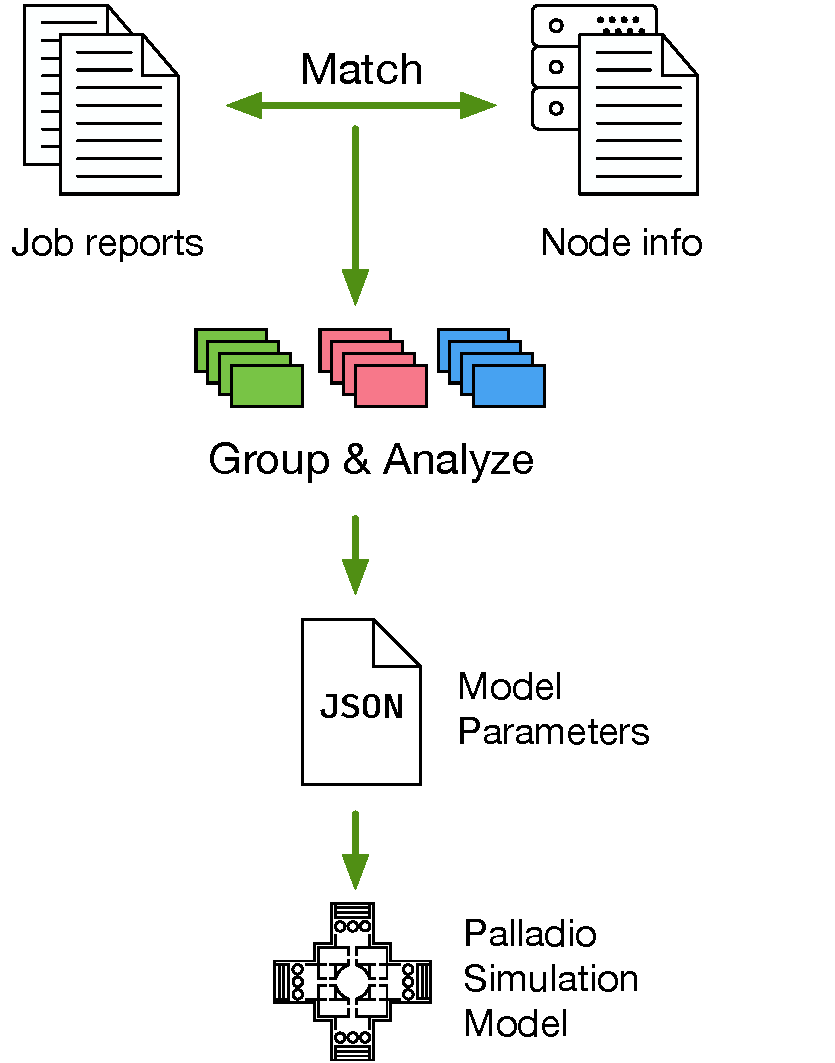
\includegraphics[width=0.8\textwidth]{Bilder/model-parameter-process.pdf}
            \end{center}   
        \end{column}

    \end{columns}
    
\end{frame}



\section*{Validation}
\begin{frame}
\frametitle{Validation}
\begin{columns}
	\begin{column}{0.45\textwidth}
		\begin{itemize}
			\item  Simulation of CMS computing jobs at GridKa for one week. 
				Based on measured data from April 2018.
			\item Metrics
		    \begin{itemize}
		    	\item Throughput
		    	\item Share of job types
		    	\item CPU efficiency
		    \end{itemize}
	    	\item High accuracy
		\end{itemize}
		\begin{center}
		\end{center}
	\end{column}
	\begin{column}{0.45\textwidth}
				
		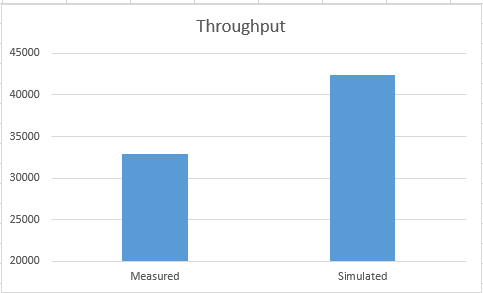
\includegraphics[width=\textwidth]{Bilder/durchsatz}
		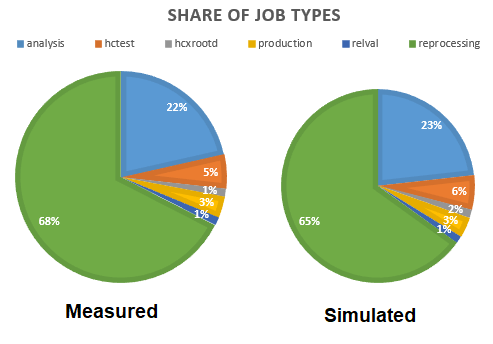
\includegraphics[width=\textwidth]{Bilder/shares}

	\end{column}
\end{columns}
\end{frame}


\note[itemize]{
	\item Required time to simulate one week is 18min.
	\item To simulate the effect of pilot draining a delay was introduced.
	Each job waits after it finished until a new job starts, to match the measured throughput.
}

\section*{Outlook}
\begin{frame}[c]
\frametitle{Conclusion}
\begin{itemize}
    \item Computing resources for user analyses will become \alert{increasingly distributed and heterogeneous} in the future
    \item Scheduling will be a key component for the \alert{efficient usage}
    \item In cooperation with computer scientists at KIT use the tool Palladio to \alert{model and evaluate different scheduling strategies}
    \item A \alert{proof of concept} for the usage of Palladio was performed simulating CMS workflows at the Tier 1 center GridKa
    \begin{itemize}
        \item Fully automated model creation based on data from CMS workflow monitoring and GridKa
        \item We were able to successfully model the situation at GridKa for key metrics
        \item Investigate how to model further metrics
    \end{itemize}
    \item Extend the current model to be able to \alert{include distributed heterogeneous computing resources}

\end{itemize}

\end{frame}


\end{document}
